
% ----------------------------------------------------------
\chapter{Metodologia de calibração utilizando as leituras de todos os sensores}\label{cap:calib-methodology}
% ----------------------------------------------------------

No Capítulo \ref{cap:field-monit-results} foram apresentados os resultados de aplicar modelos de regressão nas leituras dos sensores de gases para inferir a concentração real de cada poluente. Neles foram consideradas como variáveis de entrada de cada modelo a temperatura e as leituras do(s) sensor(es) especificados para cada composto gasoso. Assim, foram utilizados um sensor CO-B4 e a temperatura para medir \acrshort{co}; dois sensores OX-B431 e a temperatura para medir \acrshort{o3}; e um sensor NO2-B43F para medir \acrshort{no2}. No presente capítulo, serão aplicada uma metodologia de calibração similar ã do capítulo \ref{cap:field-monit-results}, mas dessa vez serão consideradas as leituras de todos os sensores para inferir a concentração de cada gás. Serão aplicadas buscas em grid para avaliar as combinações de variáveis de entrada e de parâmetros que produzam os melhores resultados de R2 e erro. Como a complexidade dos modelos aumenta com o incremento das variáveis independentes, também serão considerados as métricas de \acrshort{aic} e \acrshort{bic} na avaliação dos modelos de regressão.

\section{Calibração das leituras de \acrshort{co}}

A Figura \ref{fig:data-co-all-models-performance} apresenta os valores de R2 dos 10 melhores modelos de calibração calculados para as leituras de \acrshort{co}. Observa-se que apesar do valor médio de R2 obtido nas validações cruzadas continuar sendo negativo, obtiveram-se máximos de aproximadamente 0.1 para alguns conjuntos de dados ao utilizar regressões com k vizinhos mais próximos considerando as leituras de \acrshort{o3} e \acrshort{mp10}.

\begin{figure}[h]
    \centering
    \caption{Resultados dos 10 melhores modelos de calibração aplicados as leituras de \acrshort{co} do sensor CO-B4}
    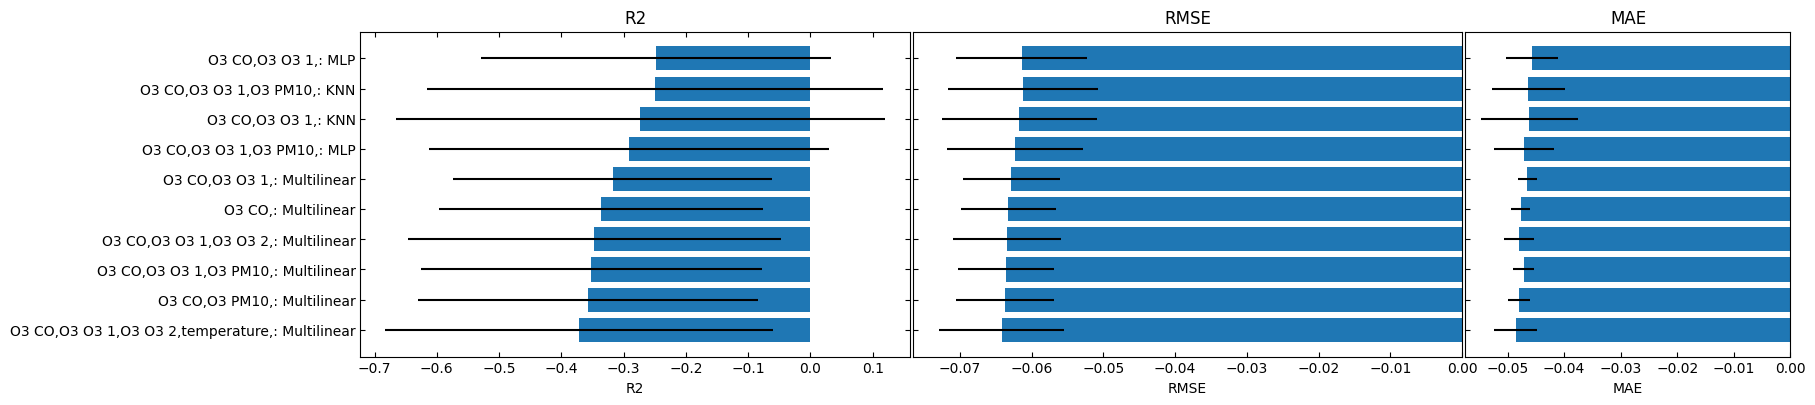
\includegraphics[width=\textwidth]{chapters/3-ANÁLISE DOS DADOS/Figuras/co-all-models-performance.png}
    \label{fig:data-co-all-models-performance}
\end{figure}

A Figura \ref{fig:data-co-all-models-comparison} mostra uma comparação do desempenho, em termos do valor médio de R2, de cada modelo de regressão aplicado para diferentes combinações de variáveis de entrada.

\begin{figure}[h]
    \centering
    \caption{Comparação dos modelos de calibração aplicados as leituras de \acrshort{co} do sensor CO-B4}
    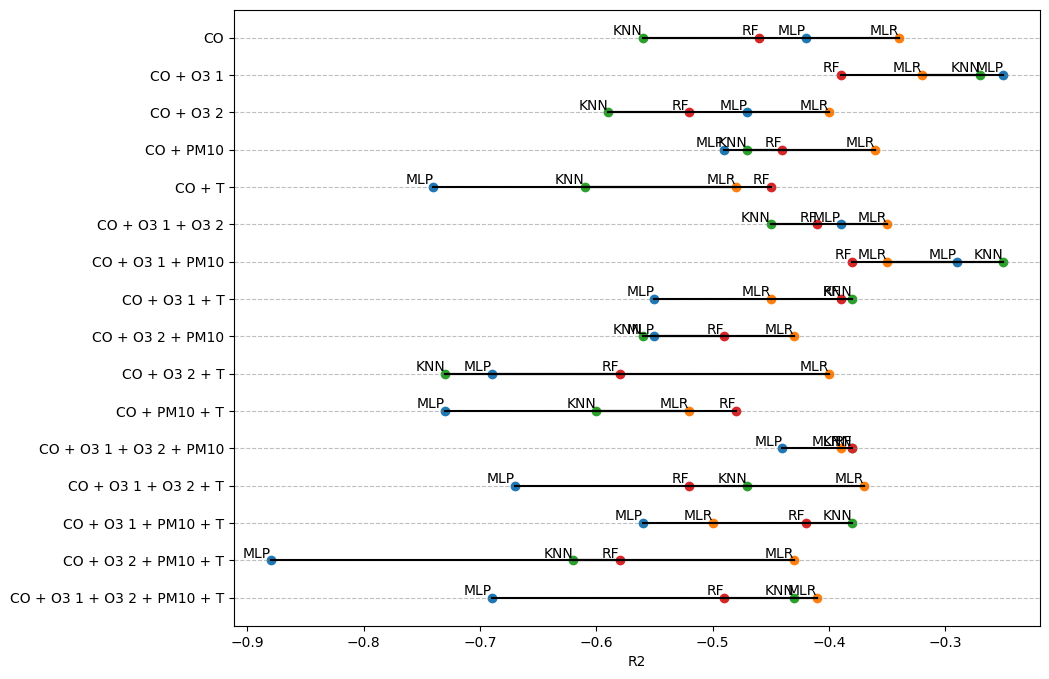
\includegraphics[width=\textwidth]{chapters/3-ANÁLISE DOS DADOS/Figuras/co-all-models-comparison.png}
    \label{fig:data-co-all-models-comparison}
\end{figure}

\section{Calibração das leituras de \acrshort{o3}}

A Figura \ref{fig:data-o3-all-models-performance} apresenta os valores de R2 dos 10 melhores modelos de calibração calculados para as leituras de \acrshort{o3}. Observa-se que apesar do valor médio de R2 obtido nas validações cruzadas continuar sendo negativo, obtiveram-se máximos de aproximadamente 0.1 para alguns conjuntos de dados ao utilizar regressões com k vizinhos mais próximos considerando as leituras de \acrshort{co} e \acrshort{mp10}.

\begin{figure}[h]
    \centering
    \caption{Resultados dos 10 melhores modelos de calibração aplicados as leituras de \acrshort{o3} do sensor OX-B431}
    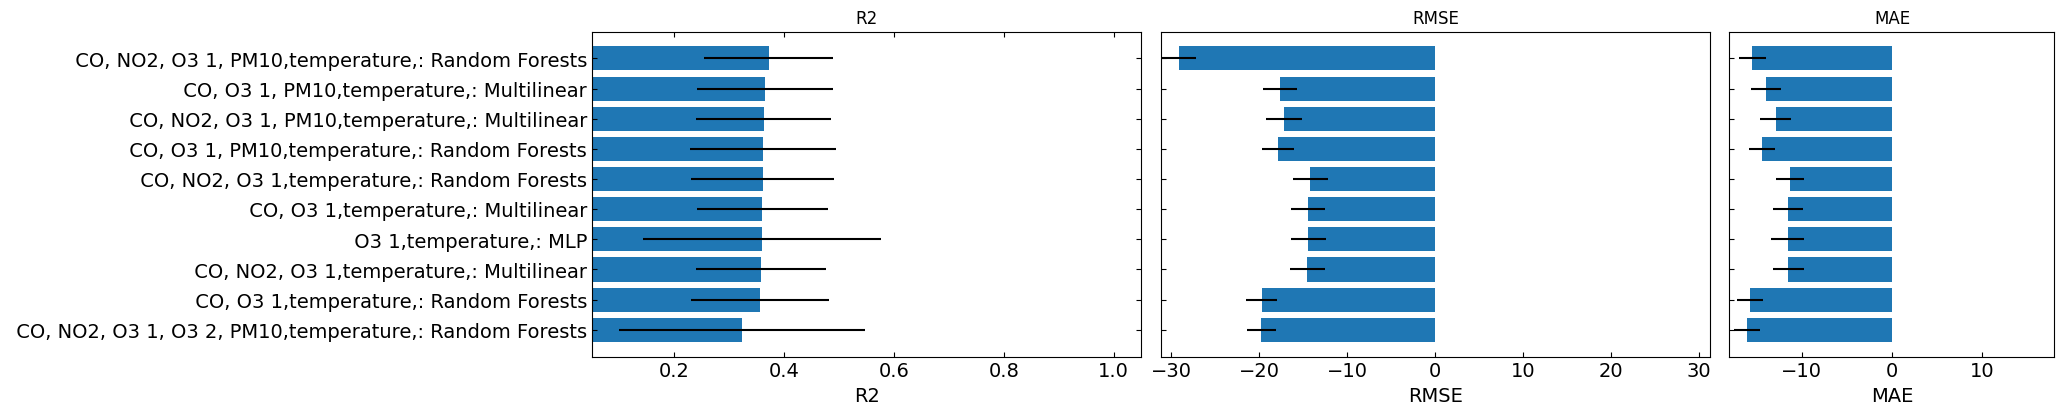
\includegraphics[width=\textwidth]{chapters/3-ANÁLISE DOS DADOS/Figuras/o3-all-models-performance.png}
    \label{fig:data-o3-all-models-performance}
\end{figure}

A Figura \ref{fig:data-o3-all-models-comparison} mostra uma comparação do desempenho, em termos do valor médio de R2, de cada modelo de regressão aplicado para diferentes combinações de variáveis de entrada.

\begin{figure}[h]
    \centering
    \caption{Comparação dos modelos de calibração aplicados as leituras de \acrshort{o3} do sensor OX-B431}
    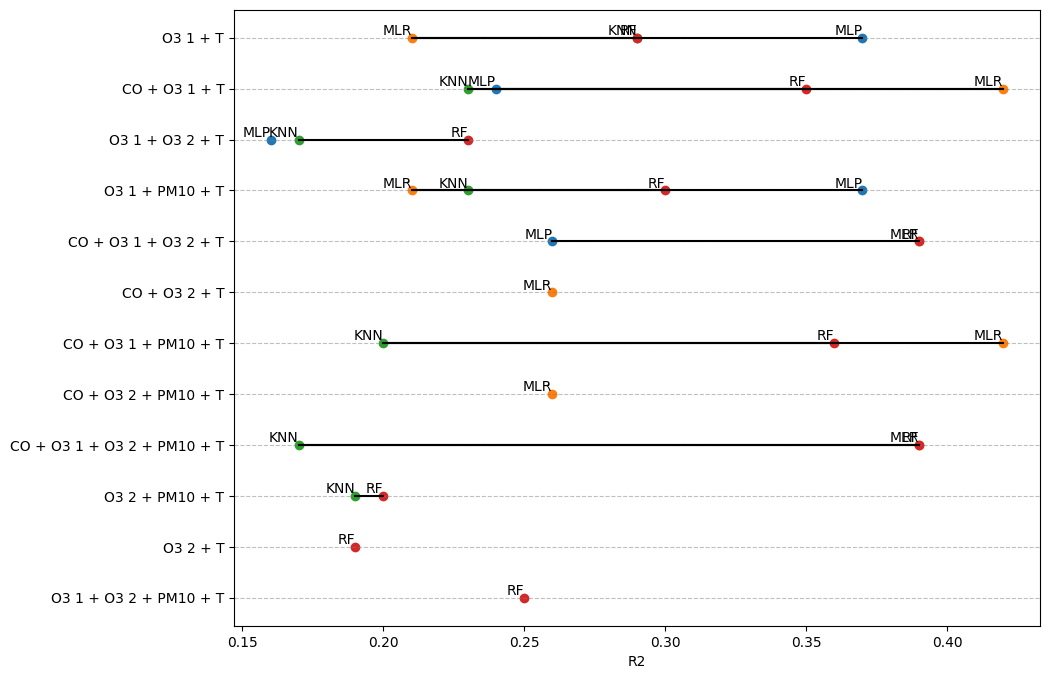
\includegraphics[width=\textwidth]{chapters/3-ANÁLISE DOS DADOS/Figuras/o3-all-models-comparison.png}
    \label{fig:data-o3-all-models-comparison}
\end{figure}

\section{Calibração das leituras de \acrshort{mp10}}

A Figura \ref{fig:data-pm10-all-models-performance} apresenta os valores de R2 dos 10 melhores modelos de calibração calculados para as leituras de \acrshort{mp10}. Observa-se que apesar do valor médio de R2 obtido nas validações cruzadas continuar sendo negativo, obtiveram-se máximos de aproximadamente 0.1 para alguns conjuntos de dados ao utilizar regressões com k vizinhos mais próximos considerando as leituras de \acrshort{o3} e \acrshort{mp10}.

\begin{figure}[h]
    \centering
    \caption{Resultados dos 10 melhores modelos de calibração aplicados as leituras de \acrshort{mp10} do sensor OPC-N3}
    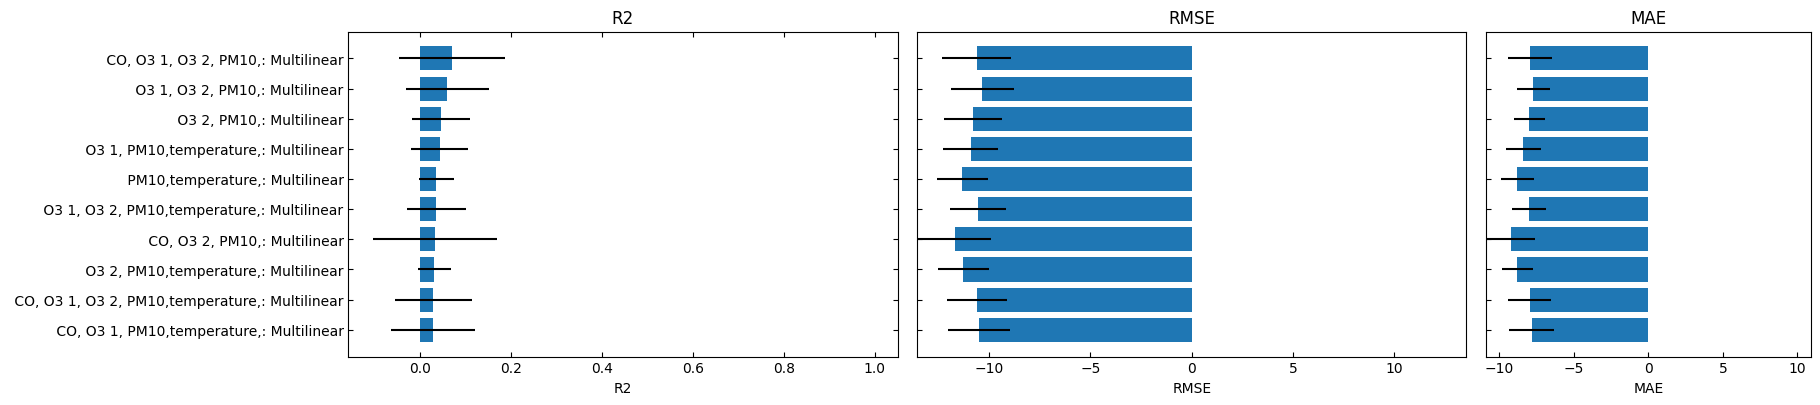
\includegraphics[width=\textwidth]{chapters/3-ANÁLISE DOS DADOS/Figuras/pm10-all-models-performance.png}
    \label{fig:data-pm10-all-models-performance}
\end{figure}

A Figura \ref{fig:data-pm10-all-models-comparison} mostra uma comparação do desempenho, em termos do valor médio de R2, de cada modelo de regressão aplicado para diferentes combinações de variáveis de entrada.

\begin{figure}[h]
    \centering
    \caption{Comparação dos modelos de calibração aplicados as leituras de \acrshort{mp10} do sensor OPC-N3}
    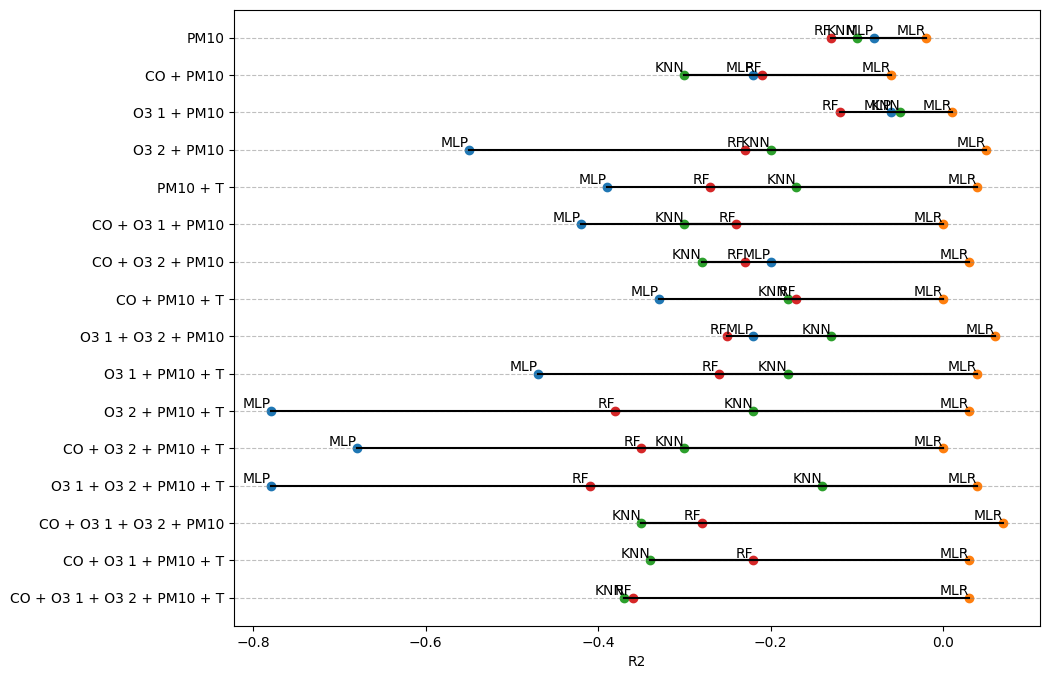
\includegraphics[width=\textwidth]{chapters/3-ANÁLISE DOS DADOS/Figuras/pm10-all-models-comparison.png}
    \label{fig:data-pm10-all-models-comparison}
\end{figure}
